\chapter{Optimization of \protect\\ Falling and Landing Motions}

This section descries algorithm for generating natural and safe
falling and landing motions of virtual and real humanoids.
First, we develop an online algorithm for simulated characters
to generate natural falling and landing motions from different 
heights and initial conditions, while absorbing impact.
In addition, we investigate a scenario of safe falling 
strategy for robots to protect themselves from large external 
perturbations by executing breakfall techniques.

\section{Falling and Landing Motion Control for A Virtual Character}

We introduce a new method to generate agile and natural human landing
motions in real-time via physical simulation without using any mocap
or pre-scripted sequences. We develop a general controller that allows
the character to fall from a wide range of heights and initial speeds,
continuously roll on the ground, and get back on its feet, without
inducing large stress on joints at any moment. The character's motion
is generated through a forward simulator and a control algorithm that
consists of an airborne phase and a landing phase. During the airborne
phase, the character optimizes its moment of inertia to meet the ideal
relation between the landing velocity and the angle of attack, under
the laws of conservation of momentum. The landing phase can be divided
into three stages: impact, rolling, and getting-up. To reduce joint
stress at landing, the character leverages contact forces to control
linear momentum and angular momentum, resulting in a rolling motion
which distributes impact over multiple body parts. We demonstrate that
our control algorithm can be applied to a variety of initial
conditions with different falling heights, orientations, and linear
and angular velocities. Simulated results show that our algorithm can
effectively create realistic action sequences comparable to real world
footage of experienced freerunners.

\begin{figure}[htbp]
\center
  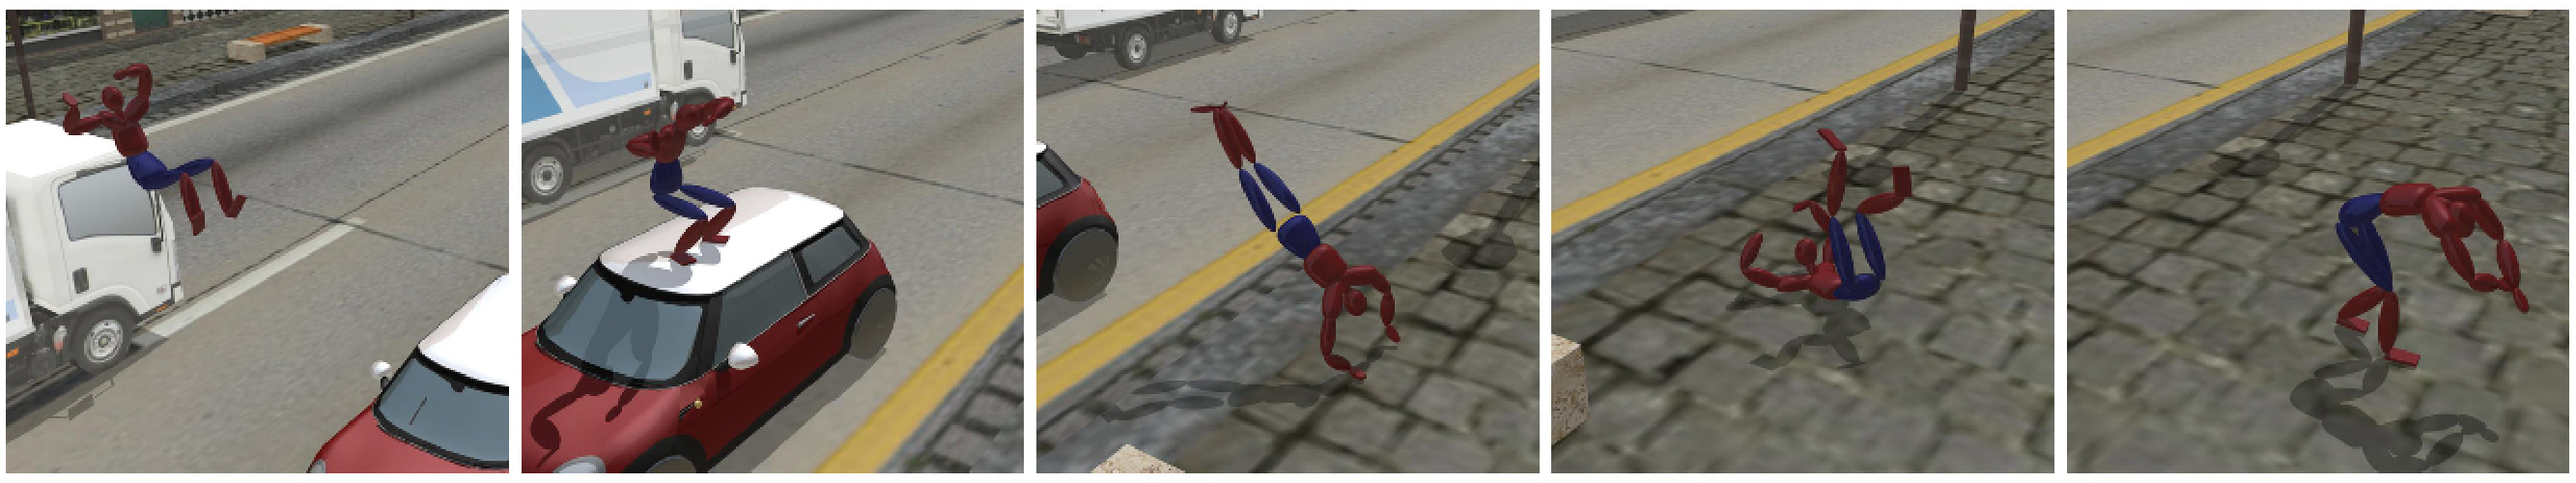
\includegraphics[width=\linewidth]{images/falling1_teaser}
  \caption{A simulated character lands on the roof of a car, 
    leaps forward, dive-rolls on the sidewalk, 
    and gets back on its feet, all in one continuous motion.}
 \label{fig:landingOverview}
\end{figure}


\subsection{Algorithm}

\subsection{Results}

\section{Multi-contact Falling Motion Control for a Humanoid Robot}
